\documentclass[conference,compsoc]{IEEEtran}



% *** CITATION PACKAGES ***
%
\ifCLASSOPTIONcompsoc
  % IEEE Computer Society needs nocompress option
  % requires cite.sty v4.0 or later (November 2003)
  \usepackage[nocompress]{cite}
\else
  % normal IEEE
  \usepackage{cite}
\fi
% cite.sty was written by Donald Arseneau
% V1.6 and later of IEEEtran pre-defines the format of the cite.sty package

%######### citações modelo abnt 2 ############
\usepackage[num]{abntex2cite}


% *** GRAPHICS RELATED PACKAGES ***
%
\ifCLASSINFOpdf
   \usepackage[pdftex]{graphicx}
  % declare the path(s) where your graphic files are
   \graphicspath{{../pdf/}{../jpeg/}}
  % and their extensions so you won't have to specify these with
  % every instance of \includegraphics
   \DeclareGraphicsExtensions{.pdf,.jpeg,.png}
\else
  % or other class option (dvipsone, dvipdf, if not using dvips). graphicx
  % will default to the driver specified in the system graphics.cfg if no
  % driver is specified.
   \usepackage[dvips]{graphicx}
  % declare the path(s) where your graphic files are
   \graphicspath{{../eps/}}
  % and their extensions so you won't have to specify these with
  % every instance of \includegraphics
   \DeclareGraphicsExtensions{.eps}
\fi

\usepackage{graphicx} % para EPS
\usepackage{subfig}

% correct bad hyphenation here
\hyphenation{op-tical net-works semi-conduc-tor}

% Acentuação Português do Brasil
\usepackage[utf8]{inputenc}

% Permite que o \LaTeX\ fale em português
\usepackage[brazil]{babel}

%hiperlink de Internet
\usepackage[pdftex]{hyperref}


% Conta o número de páginas
\usepackage{lastpage}
\usepackage{setspace}
\pagestyle{plain}

\begin{document}
%
% paper title
% Titles are generally capitalized except for words such as a, an, and, as,
% at, but, by, for, in, nor, of, on, or, the, to and up, which are usually
% not capitalized unless they are the first or last word of the title.
% Linebreaks \\ can be used within to get better formatting as desired.
% Do not put math or special symbols in the title.
\title{Minerando dados em grandes quantidades - \textit{Big Data}: SURVEY}


% author names and affiliations
% use a multiple column layout for up to three different
% affiliations
\author{\IEEEauthorblockN{Othon L. T. Oliveira}
\IEEEauthorblockA{Mestrando em Engenharia de Sistemas\\
Universidade de Pernambuco\\
Email: olto@ecomp.poli.br}
\and
\IEEEauthorblockN{Fernando B. L. Neto}
\IEEEauthorblockA{Universidade de Pernambuco\\PhD - UK\\
Email: fbln@ecomp.poli.br}
}

% conference papers do not typically use \thanks and this command
% is locked out in conference mode. If really needed, such as for
% the acknowledgment of grants, issue a \IEEEoverridecommandlockouts
% after \documentclass


% make the title area
\maketitle

% As a general rule, do not put math, special symbols or citations
% in the abstract
\begin{abstract}
Este artigo pretende fazer uma explanação de um novo paradigma; o paradigma da informação ilimitada, conhecido como "Big Data" e, propor uma solução para recuperação de informação para grandes espaços de buscas. Atrelado à este paradigma e, reforçando o conceito de que uma nova onda está à frente para a Internet, onde coisas se conectam com coisas, conhecida como Internet das coisas ou simplesmente IoT. A Internet das coisas é também conhecido como a "terceira onda da Internet", o entendimento seria algo como; computadores conectados a eletrodomésticos; telefones celulares ligados à semáforos, recebendo informações sobre o tempo, acidentes e congestionamento e, passar esta informação ao carro, que avisa o condutor que está à frente. Esta é a realidade que se aproxima e pretendemos analisar neste artigo como os novos ``atores'', ou coisas interagem com os atores humanos tradicionais.
\end{abstract}

\vspace{0.1cm}

\textit{\textbf{Palavras-chave: Big Data, Mapear e Reduzir, Hadoop, Enxame de robôs, Inteligência em enxames, Aprendizado em profundidade, Aprendizado de máquina, Otimização por enxame de partículas, Otimização por enxame de formigas, Pesquisa por cardume de peixes, Logística, Roteamento }}.

\vspace{0.1cm}

\textit{Abstract -- This paper intends to make an explanation of a new paradigm, the paradigm of unlimited information known as "Big Data" and to propose a solution for information retrieval for large spaces searches. Coupled to this paradigm and, reinforcing the concept that a new wave lies ahead for the Internet, where things connect with things, we are not as well known Internet of Things   or simply IoT. The IoT is also known as the "third wave of the Internet," the acronym is confirmed because something like computers connected to home appliances, mobile phones connected to the traffic lights, getting weather information, accidents and congestion and to pass this information to the car, which warns the driver what's ahead. This is the reality that approaching and we intend to analyze in this article how the new players, things, interact with traditional actors humans.}

\textit{Keywords: Big Data, Map Reduce, Hadoop, Swarm Robotics, Swarm Intelligence, Deep Learning, Machine Learning, Particle Swarm Optimization, Ant Colony Optimization, Fish School Search, Logistic, Routing}.



% For peer review papers, you can put extra information on the cover
% page as needed:
% \ifCLASSOPTIONpeerreview
% \begin{center} \bfseries EDICS Category: 3-BBND \end{center}
% \fi
%
% For peerreview papers, this IEEEtran command inserts a page break and
% creates the second title. It will be ignored for other modes.
\IEEEpeerreviewmaketitle



\section{Introdução}

Inferir sobre algum assunto agora poderá ser coisa do passado. Astrônomos atualizam suas descobertas numa base de 
dados disponíveis para outros utilizarem, as ciências biológicas agora tem tradição em depositar seus avanços 
científicos em repositórios públicos, redes sociais estão focadas na Web; Facebook, 
LinkedIn, Microsoft, Tweeter e Yahoo sobrevivem coletando informações e repassando-as as empresas de telemarketing, 
empresas de comércio eletrônico como Amazon, Submarino, Americanas.com, Magazine Luiza, utilizam essas informações 
para vender mais e melhor, artigos científicos dos mais variados assuntos, das mais variadas áreas alimentam, 
todos os dias,  com milhões de informações os \textit{Data Centers}, isso é o \textit{Big Data}.


Para fazer frente a esse novo paradigma e extrair informações com eficiência uma nova abordagem algorítmica se faz necessário. 
As técnicas tradicionais de busca tradicionais não são eficientes para resolver muitos problemas com grande complexidade, i.e. ordens de grandeza 
dantes inimagináveis, especialmente as que possuem complexidade exponenciais, geradas por explosões combinatórias, felizmente, 
muitos desses problemas não-triviais são eficientemente resolvidos por soluções naturais \cite{Swarm_Medeiros}.

Para resolver a problemática da explosão combinatória de informações, são desenvolvidas técnicas para reduzir o tempo de busca, 
tornando os custos computacionais mais aceitáveis, na medida que não exploram todas as possibilidades no caminho até a 
solução procurada, somente o caminho curto onde é mais provável de se encontrar a solução, a essa técnica dá-se o nome de heurística.

As meta-heurísticas são soluções encontradas nas mais diversas espécies de seres vivos, por exemplo, as formigas quando 
vão em busca de alimentos, facilmente encontram um caminho mais curto entre o ninho e a fonte de alimentos, cardumes de peixes 
executam movimentos aparentemente aleatórios mas, quando em grupo, são precisos para fuga dos predadores, bandos de pássaros 
quando em busca de novos locais para ninhos ou de alimento, inspiram os mais diversos algoritmos inteligentes baseados em 
populações de animais sociáveis, demonstrando que há uma inteligência coletiva nessas populações, desenvolvida ao longo do 
tempo e das interações entre essas espécies sociáveis e o meio ambiente. Essa classe de algoritmos, metaforiza o comportamento 
de tais populações, e promoveu o desenvolvimento de uma área que hoje é conhecida como computação bio inspirada ou computação 
natural. Essa área investiga a relação entre a computação e a biologia (e mesmo a sociologia), estudando soluções de buscas 
e otimização, modelando problemas mais eficientemente, baseado nas elegantes soluções encontradas pela natureza.


\section{Objetivos}

Este artigo ``Survey'' tem como objetivo analisar a problemática do Big Data e seus paradigmas apresentados atualmente, os 5 V's, extrair informações dele para propor solução à logística de cargas aplicada `a realidade das rodovias brasileiras, objetivando assim uma alternativa ao traçado de rotas determinísticas, inspirado em buscas no \textit{Big Data}. 



\section{Plano de execução do Survey}

Para executarmos este \textit{Survey}, foram primeiramente definidas as seguintes etapas:

\begin{enumerate}
 \item[A.] Coleta dos dados;
 \item[B.] Seleção dos artigos; 
 \item[C.] Escolha dos Filtros;
 \item[D.] Leitura dos artigos.
\end{enumerate}

\begin{enumerate}
 \item[A.] Coleta dos dados\\
 Para coletar os dados foram escolhidas sete (7) palavras chaves com relevância ao tema dentro do meio ambiente da pesquisa, destacamos:
  \begin{itemize}
    \item “Data Mining and Swarm Intelligence”
    \item “Data Mining Big Data”
    \item “Data Mining Swarm Robotics”
    \item “Deep Learning”
	\item “Hadoop Map Reduce in Big Data”    
    \item "Machine Learning"
    \item “Map Reduce Big Data”
  \end{itemize}


 De posse das palavras-chave foram criadas planilhas, onde cada folha dessa planilha é representada por uma palavra chave. 
 Incluiu-se no mínimo 30 artigos para cada planilha. 
 Pretendeu-se, com essa arquitetura, construir rapidamente gráficos das mais diferentes matizes, tais como:
  \begin{itemize}
    \item Base pesquisada;
    \item Data da publicação do artigo;
    \item Aceito ou rejeitado;
    \item Título do artigo;
    \item País de origem do artigo.
  \end{itemize}

  Uma das ferramentas utilizadas para extrair os dados referentes às palavras-chave foi o programa Mendeley, especializado
  em extrair dados de arquivos pdfs como os artigos, dissertações e teses. O Mendeley oferece uma opção para gerar dados 
  extraídos em formato estruturado do tipo XML. A priori foi utilizado para gerar as planilhas, contudo, foi excluída essa
  opção por não trazer grandes ganhos, talvez se fossem criadas macros para tratar esses arquivos XML ficassem mais ``limpos''
  pois o que mais foi relevante para esta fase do Survey formaram as colunas de cada planilha:
  A figura 1 mostra como está a planilha-Survey até este momento;
  
 
  \begin{figure}[!ht]
  \centering %\centering % para centralizarmos a figura
  \caption{Planilha}
  \flushright
  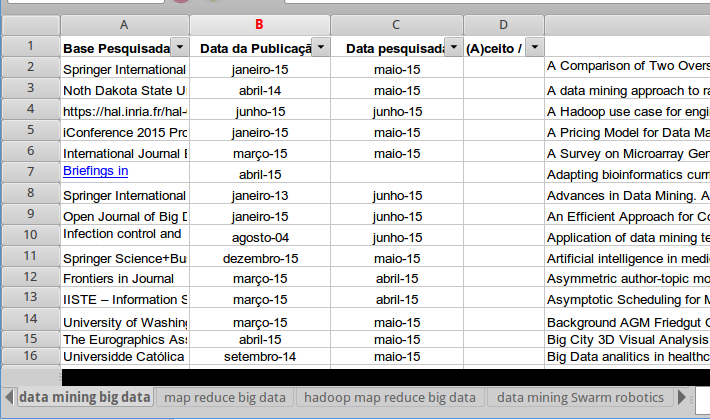
\includegraphics[width=0.4\textwidth]{Figuras/PlanilhaSrvey.png}
%  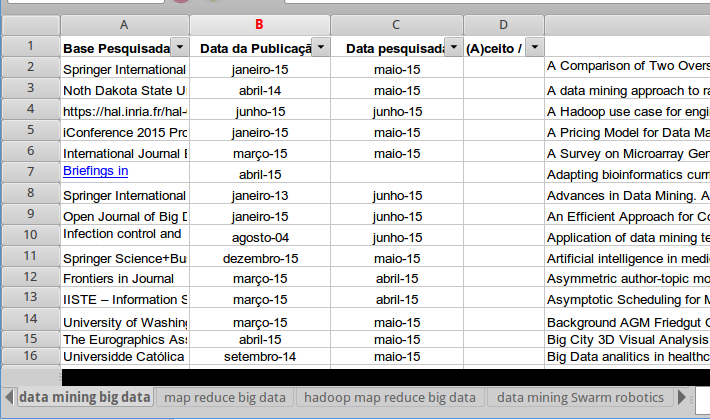
\includegraphics[scale=0.35]{Figuras/PlanilhaSrvey.png}
%  \label{Fig 1}
  \end{figure}
  
  \item[B.] Seleção dos artigos\\
  A seleção dos artigos foi primeiramente escolhida de forma qualitativa, pelas mais recentes publicações, 
  dos últimos 5 anos, para ser mais exato entre 2010 e 2015. O segundo critério de seleção foi pelo órgão publicizador, 
  haja vista os mais conhecidos tais como IEEE, Elsevier, Springer, e deles todos os jornais pertinentes, contudo
  outras fontes foram consideradas como universidades, seminários mais conhecidos na área.

  Outro critério de seleção foi o quantitativo. Para isso foi estabelecido o mínimo de 30 (trinta artigos) por palavra chave.
  Dessa forma procuramos aproximar os dados coletados da distribuição normal padrão que por razões evidentes está amplamente
  tabelada e é suprida por quase todos os software para construtores de gráficos.\\

  \item[C.] Critérios de Inclusão/Exclusão \\
  O critério de inclusão e exclusão foi baseado na leitura dos ``abstracts'' dos artigos. 
  Devido a algumas palavras estarem muito na ``moda'' são citados em muitos artigos, apesar de conterem as palavras chaves,
  mesmo assim não traziam qualquer relevância para a pesquisa. Dessa forma foi criada uma pasta chamada “Rejeitados” 
  para onde foram movidos esses artigos.\\
  Outro critério de exclusão foi a data mais antiga, anteriormente à 2010, com alguma exceção dos artigos clássicos da área.\\

  \item[D.] Leitura dos artigos \\
  A leitura dos artigo iniciou-se tão logo terminaram os critérios de de Inclusão/Exclusão.
  Foram selecionados cerca de 100 artigos para serem lidos, não excetuando-se excluir mais algum que por ventura não 
  tenham ficados ``presos'' na etapa anterior (C), dos filtros.
  Segue uma tabela com as datas do plano de execução
  
  \begin{table}[htbp]
  \scriptsize
  \centering
  \caption{Datas do Survey}
  \begin{tabular}{|p{18mm}|p{8mm}|p{8mm}|p{8mm}|}
  \hline
  Data & A-Coleta & B-Seleção & C-Filtros \\
  \hline
  Abril a Junho & X & -- & -- \\ \hline
  Junho e Julho & -- & X & X \\ \hline
  Agosto & -- & -- & X \\ \hline

  \end{tabular}
  \end{table}


\end{enumerate}

\section{A Internet}

Uma \textit{Internetwork} ou simplesmente internet é a conexão entre mais de uma rede e hoje em dia a maioria das redes se encontram conectadas.  A Internet é um sistema de \textit{internetwork} organizado e estruturado, a mais notável das internets, uma colaboração de mais de centenas de milhares de redes. Já ``World Wide Web'' (WWW) é apenas um dos muitos serviços que funcionam dentro da Internet. 

O acesso à Internet está condicionado a Provedores de Acesso (ISP), que se classificam em internacionais, que conectam países; nacionais (\textit{backbones} criadas e mantidas por empresas especializados) ; regionais ligadas a outros ISPs, normalmente têm taxas de transmissão menores; e locais que se conectam a ISP regionais ou nacionais e oferecem serviços de conexão a usuários finais.


\begin{figure}[!h]
\centering
%\centering % para centralizarmos a figura
\caption{Internet}
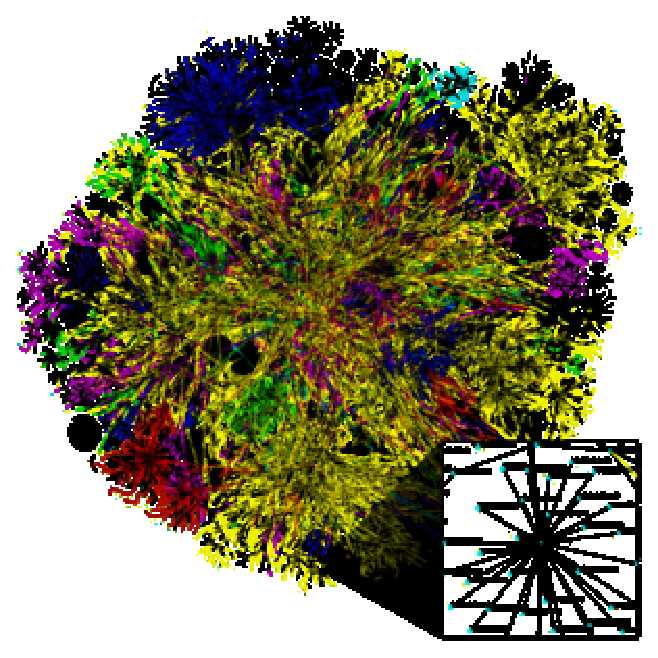
\includegraphics[width=50mm]{Figuras/internet_map.eps}
%\label{figura 2}
\end{figure}



\subsection{Redes de dispositivos conectados}
% no \IEEEPARstart
Uma rede é um conjunto de dispositivos (nós) conectados por links (caminho de transferência) de comunicação.  Um nó pode ser um computador, uma impressora ou outro dispositivo de envio e/ou recepção de dados, que estejam conectados a outro nó da rede \cite{Forouzan}.

Por mais simples e menor que seja, três critérios são considerados os mais importantes que uma rede deve atender: Desempenho, que envolve a capacidade de vazão (througput) e o atraso (delay); Confiabilidade, que envolve o tempo de recuperação quando falha e sua robustez caso haja alguma catástrofe; e Segurança, que envolve proteção ao acesso de dados e proteção contra danos e perdas \cite{Forouzan} \cite{Specialski}.



\section{Big data}

"Em 2010 empresas e usuários armazenaram mais de 13 exabytes de novos dados" \cite{bigdataQualquerUm}.

Atrelada a essa produção massiva de dados, uma nova onda está sendo vislumbrada, é chamada de ''A terceira onda da Internet''
, onde coisas se conectam com coisas; produtos nas gôndolas do supermercado com um novo tipo de etiqueta se conectam a uma 
leitora de radio frequência à alguns metros de distância, contabilizando o total do estoque em segundos; o consumidor leva 
seus produtos escolhidos ao caixa desse supermercado, pagando a conta sem precisar retirar qualquer produto do carrinho. 
Ao introduzir esses produtos na geladeira, será possível saber quando expira a data de validade de determinados produtos, sem 
precisar abri-la, e quando acabarem esses produtos, a própria geladeira informará ao supermercado a falta deles, reservando 
o próximo rol de compras. Assim será essa onda de coisas conectadas, chamada de Internet das Coisas ou \textit{Internet of Things} (IoT),
que fará com que os dados no \textit{Big Data} sofram explosão combinatória de informações multiplicando exponencialmente as dimensões deste.


O paradigma dos 5 V’s é descrito como: Volume de dados; Velocidade para acessar esses dados; 
Variedade de informações; Veracidade nos dados encontrados e Valor atribuído aos dados. 
Dentre as mais diversas ferramentas existentes destacamos algumas já consagradas como Map Reduce, da ``framework'' Hadoop,
e sua congênere desenvolvida pelo Google. Essas são as mais conhecidas dos ``aventureiros'' que estão desbravando o Big Data. Não será uma tarefa trivial inferir e desenvolver novas ferramentas, pois o Big Data tem 
assumido, nos mais recentes anos proporções gigantescas como descrito na tabela 1


%Tabela 1


\begin{table}[!ht]
\scriptsize
\centering
\caption{Volume de dados no mundo}
\begin{tabular}{|p{6mm}|p{5mm}|p{16mm}|p{8mm}|}
\hline
Ano & Qtd & Unidade & Múltiplo \\
\hline
2000 & 800 & terabytes – TB & $10^{12}$ \\ \hline

2006 & 160 & petabytes – PB & $10^{15}$ \\ \hline

2009 & 500 & exabytes – EB & $10^{18}$ \\ \hline

2012 & 2,7 & zettabytes – ZB & $10^{21}$ \\ \hline

2020 & 35 & yottabytes – YB & $10^{24}$ \\ \hline

\end{tabular}
\end{table}

As redes sociais são um arcabouço de informações sobre todo tipo de assunto vivenciado pelas pessoas, inclusive situações que dizem respeito ao nosso ambiente de pesquisa.
O cenário abaixo, encontrado numa rede social, exemplifica a sequência de informações retiradas do Twitter.
O Twitter é uma rede social, onde os usuários escrevem num pequeno espaço com cerca de 140 caracteres, os mais diversos assuntos. A ideia inicial do Twitter era que se comportasse como um ``SMS da Internet'' \cite{Twitter2015}. As informações são enviadas aos usuários, conhecidas como twittes, em tempo real e, também enviadas aos usuários seguidores que tenham assinado para recebê-las. A seguir pode-se verificar uma sequência de twittes da Polícia Rodoviária Federal de Santa Catarina:

\begin{figure}[!ht]
\caption{Twitter	}
	\subfloat[Twitte - 1 \label{subfig-1:dummy}]{%
		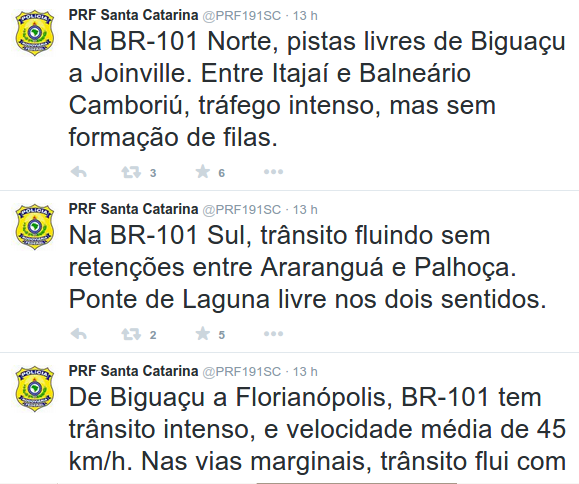
\includegraphics[width=60mm, height=70mm]{Figuras/twittePRF.png}
	}
	\quad \quad \quad \quad
	\subfloat[Twitte - 2\label{subfig-2:dummy}]{%
		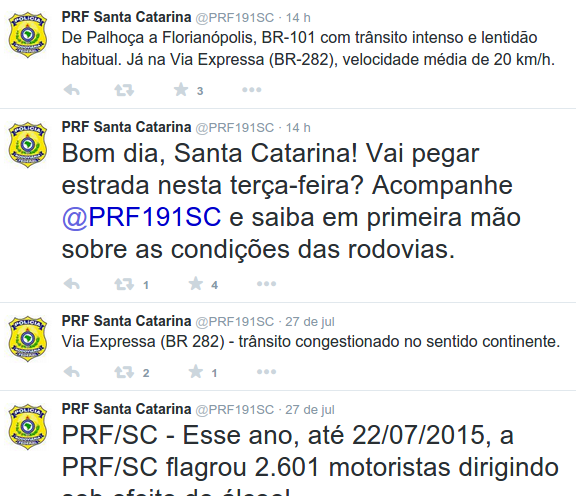
\includegraphics[width=60mm, height=70mm]{Figuras/twittePRF2.png}
	}
	\label{fig:twitter}
\end{figure}

A Polícia Rodoviária Federal de Santa Catarina, disponibilizou às 13hs através do canal @PRF191SC, informações relevantes sobre o trânsito naquela localidade, 
num universo temporal variado, por exemplo: entre Itajaí e Balneário Camboriú o transito está intenso, isso sugere que a frota de caminhões que acompanhamos até este local deva ter uma
rota alternativa, caso persista esta situação por muito tempo. No primeiro twitte da segunda coluna em Via Expressa (BR 282) trânsito lento com 
velocidade de 20km/h praticamente congestionado, novamente sugere que devamos ``pensar'' numa rota alternativa, caso esse congestionamento persista por muito tempo.

Outra rede social conhecida pelos condutores de veículos é o Waze. O Waze é um aplicativo de navegação para o trânsito, funciona em aparelhos celulares e tablets. Os utilizadores desse aplicativo são conhecidos como wazers, os wazers compartilham informações sobre o trânsito, em tempo real. Contudo as informações somente estão disponíveis no momento em que são postadas pelos utilizadores por um período de tempo pequeno, caso não hajam utilizadores trafegando pelas vias ou esses utilizadores não tenham disponibilidade em postar informações, não há o que se compartilhadar.
Outra problema levantado com o waze é que; caso não haja conexão à Internet não há como acessar os dados dos wazers, para navegação.

Além dos dados que chegam ao \textit{Big Data} através das redes sociais, o trânsito das grandes cidades têm disponíveis câmeras de monitoramento do trânsito nos semáforos, alguns com cobertura
por canais de televisão, câmaras de segurança próximos às rodovias também coletam informações, tudo em tempo real. Os dados desses dispositívos geralente são gravados sendo conhecidos como \textit{stream} de dados. 
Esses \textit{streams} podem estar disponibilizados na Internet em sítios eletrônicos especialmente construídos para isso, como o
< http://vejoaovivo.com.br/ > e outros.

Os dados disponibilizados pelos diversos meios de comunicação não estão em formato que possam ser utilizados imediatamente, precisam antes serem processados. Esses dados não processados são conhecidos como ``dados frios''.
O processo de tratar as informações, retirando-lhes o ``lixo''; transformando dados ``frios'' em dados ``quentes'', é um processo que tem um custo temporal elevado, devido ao volume dos dados.

Para trabalhar com os dados do Big Data foi criado um tipo arquitetura para computadores trabalharem em conjunto formando um \textit{cluster} essa arquitetura é conhecida como \textit{filesystem}\footnote{\textit{Filesystem}. ou sistema de arquivos, referem-se à forma como os dados são armazenados, organizados e acessados, pelo sistema operacional, em cada partição no disco (ou no disco inteiro)}.

O goolgle criou o \cite{Filesystem} HadDoop FileSystem (HDFS).

\subsection{Hadoop - Map Reduce - Big Data}\label{arte:palavraChave:HadoopMapReduce}

Portanto o \textit{Big Data}, devido à sua natureza, é definido como um paradigma entre as grandezas: \textbf{Velocidade}, \textbf{Variedade} e \textbf{Volume}.
O roteiro seguido pela informação desde o local onde é produzida até que possa ser utilizada é  exemplificado na imagem a seguir:

\begin{figure}[ht]
\centering
\caption{Big Data e Arquitetura Haddop}
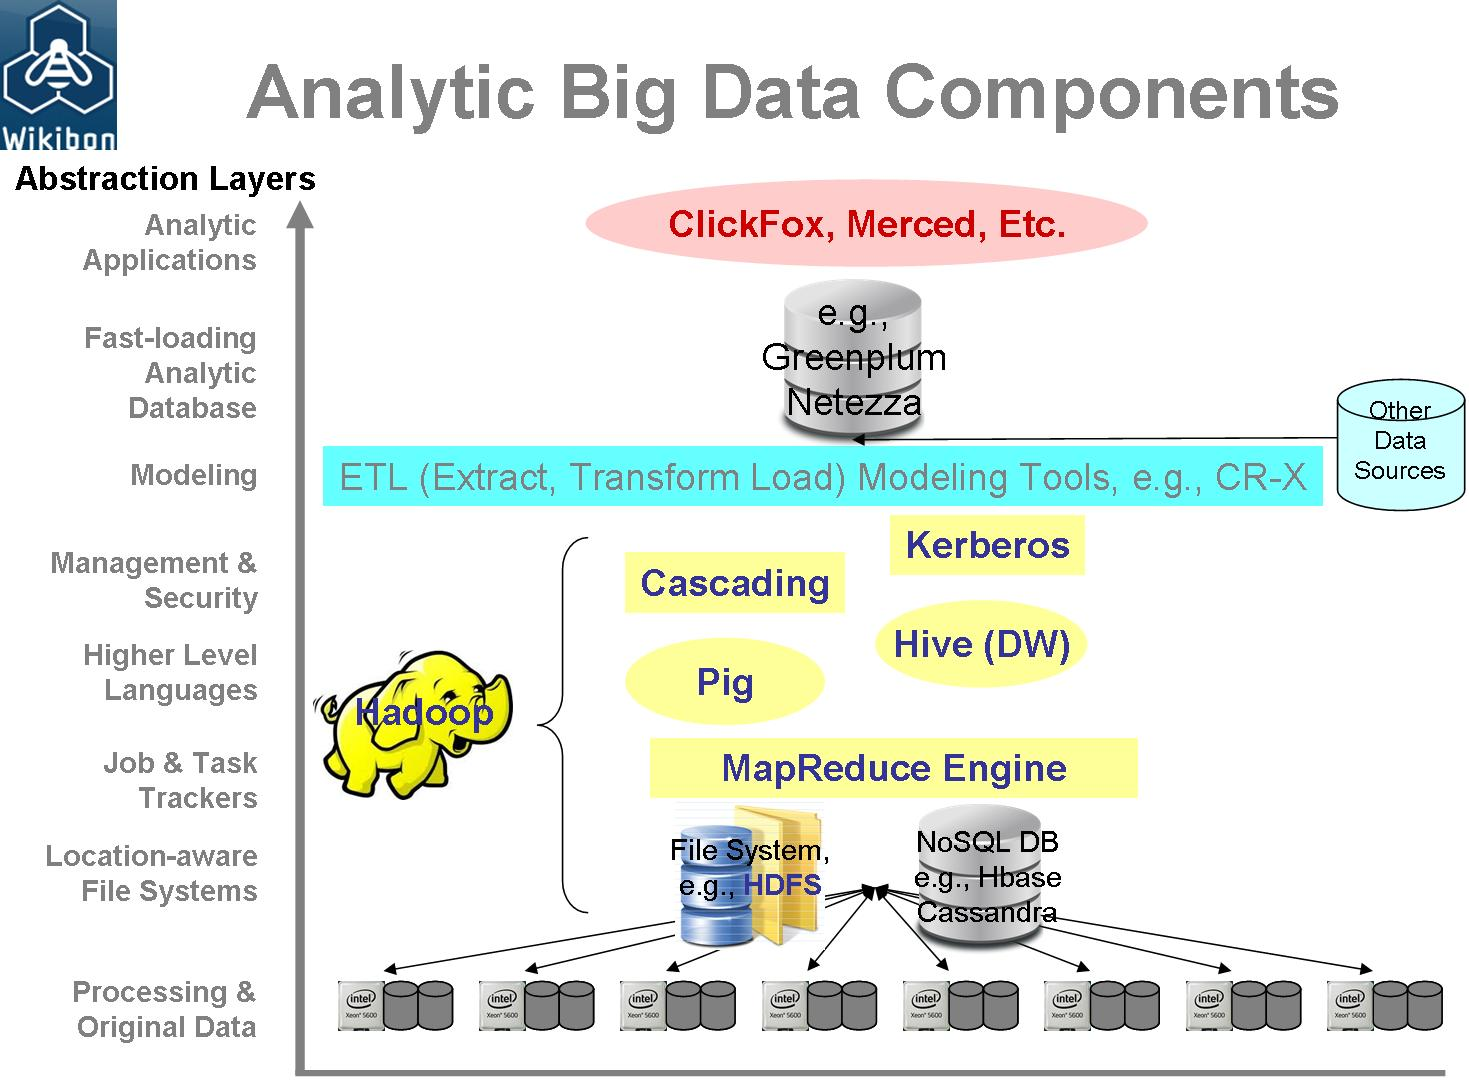
\includegraphics[width=100mm, height=80mm]{Figuras/BigDataComponents.jpg}
\end{figure}

A camada mais baixa da imagem, onde se lê \textit{Processing \& Original Data} é a origem do \textit{Big Data}, onde estão os dados ``frios''. Entre as camadas \textit{Location-aware File Systems} e \textit{Management \& Security} é o roteiro seguido pela informação para ser trasformada em dados ``quentes''. A tecnologia utilizada, neste mestrado, para tratar os dados será o Hadoop, devido ao baixo custo de implementação e por ser uma tecnologia aberta, de livre utilização, conhecida como \textit{Open Source}. O Haddop é uma arquitetura de milhares de computadores interligados e espalhados e pela Intenet. Esses computadores são especializados em extrair dados do \textit{Big Data} e transformá-los em dados relevantes (quentes). <<\textbf{citar}>>

O Haddop funciona com um agrupamento em paralelo desses computadores, conhecido como \textit{cluster}. Esse \textit{cluster} tem a característica de grande escalabilidade; em torno de 3 000 computadores, dependendo da construção, e tolerância a falhas; quando um computador do \textit{cluster} fica inoperante  ``cai'', os dados são salvos em outro computador. A estrutura de diretórios do Hadoop é conhecida como \textit{Hadoop File System} (HDFS). O HDFS foi especialmente construído para lidar com as características descritas anteriormente.



\subsection{Map Reduce - Big Data}\label{arte:palavraChave:MapReduceBigData}


O Map-Reduce é uma técnica conhecida desde a linguagem Lisp, que permite mapear o \textit{cluster} e reduzir conforme um par de informações <chave:valor>. A imagem a seguir exemplifica a técnica Map-Reduce:

\begin{figure}[ht]
\centering
\caption{Técnica Map-Reduce}
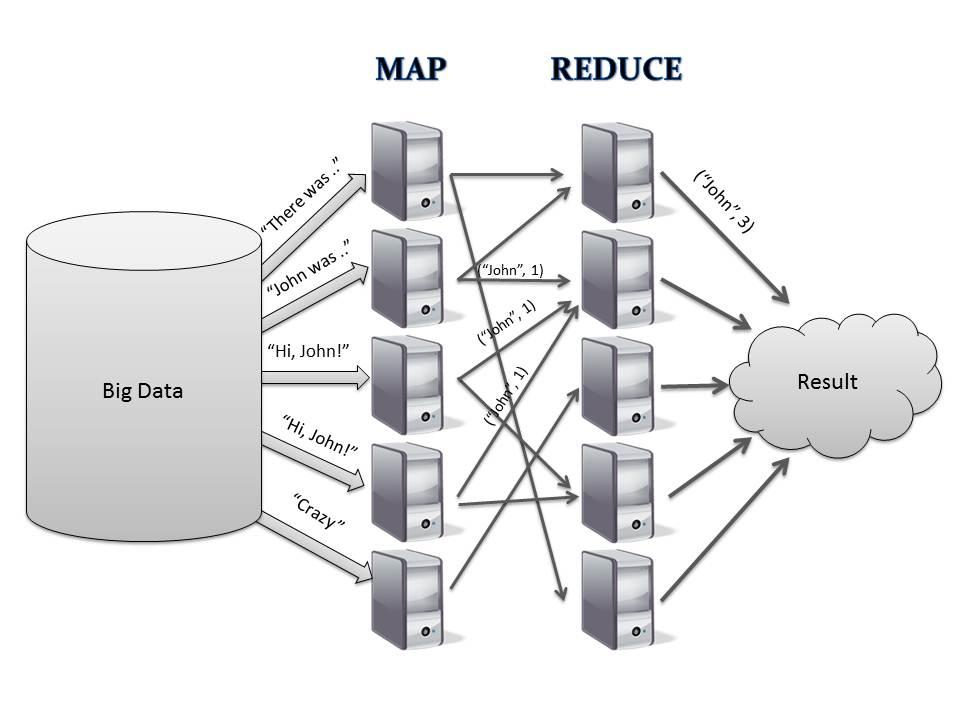
\includegraphics[width=100mm, height=80mm]{Figuras/MapReduce.jpg}
\end{figure}

Este Map-Reduce, modelo de computação paralela para ser utilizado na Internet foi proposto pelo Google
\cite{Dean2008}.

\subsection{Data Mining - Swarm Inteligence}\label{arte:palavraChave:Swarm}

\subsection{Data Mining - Big Data}\label{arte:palavraChave:DataMiningBigData}

\subsection{Data Mining - Swarm Robotics}\label{arte:palavraChave:Robotics}

O rápido crescimento da Internet, tem trazido, a reboque, o contínuo crescimento da insegurança nos computadores e sistemas \cite{Barford2007}.
Ataques utilizando à computadores através de robôs.

\subsection{Deep Learning}\label{arte:palavraChave:Deep}



\subsection{Machine Learning}\label{arte:palavraChave:Machine}

O desafio dos 3 V's (Velocidade, Variedade e Volume) pode ser um fator determinístico na escolha da ferramenta mais adequada para se analisar dados do \textit{Big Data} e extrair informação. As árvores de decisão são algorimos rápidos, contudo dados impuros podem comprometer o desepenho desse algoritmo. A fase de extração dos dados do \textit{Big Data} são fortemente influenciáveis pelas variáveis escolhidas, \cite{DecisionTree} isso pode representar o desafio maior para implementar esta técnica, na figura a seguir exemplificamos essa tarefa:

desenhar a figura

% \begin{tikzpicture}
%  \draw (0,0) -- (2,1); %reta
% \end{tikzpicture}


\section{Enxame de partículas}\label{arte:enxames}

Em 1989, G. Beni e J. Wang cunharam a expressão \textit{Swarm Intelligence}, no seu
trabalho em Robotic Swarm \cite{SRobotics}. O estudo do reino animal aprofundou-se no estudo
comportamental e possibilitou o melhor entendimento de como cooperam indivíduos dentro de um grupo e
quais os mecanismos usados para controlar o enxame e condicionar o indivíduo, tais como a estigmergia. 
Por enxame, pode entender-se manada, alcateia, bando, colônia, entre outras designações conforme o animal 
ou inseto e, a partir daqui, qualquer referência a um grupo de agentes passa a ser feita por enxame, e.g., 
um enxame de pássaros. Os 5 princípios da inteligência de enxame segundo  Chambers \cite{chambers2014computer}, são:
\begin{itemize}
	\item{Proximidade: os agentes têm que ser capaz de interagir}
	\item{Qualidade: os agentes devem ser capazes de avaliar seus comportamentos}
	\item{Diversidade: permite ao sistema reagir a situações inesperadas}
	\item{Estabilidade: nem todas as variações ambientais devem afetar o comportamento de um agente}
	\item{Adaptabilidade: capacidade de se adequar as variações ambientais}
\end{itemize}


\subsection{Particle Swarm Optimization - (PSO)}\label{arte:algo:pso}

Kennedy e Eberhart (1995), criaram a popular Otimização por Enxame de Partículas do inglês \textit{Particle Swarm Optimization} - (PSO), 
que na verdade é uma técnica de otimização de funções não-lineares baseado em populações. Foi inspirado no comportamento
social em bando de pássaros, essa técnica é uma das mais conhecidas e investigadas hoje \cite{Kennedy1995}.
Esse algoritmo (e todos os outros) têm um fator de convergência, para fazer com que encontre mais rapidamente a resposta procurada.
Para acontecer isso foi introduzido um ''poleiro'' virtual. Com essa simples abordagem foi inaugurado uma nova
família de algorítimos baseados em enxames. 

No PSO, a população é chamada enxame e os indivíduos, partículas. Cada partícula se move no espaço de busca, 
à procura de regiões promissoras; cada partícula dessas representa uma solução candidata a resolver nosso problema.
A equação utilizada para encontrar uma partícula no espaço de busca foi emprestada da cinemática:

\begin{equation}
x_i(t+1) = x_i(t) + v_i(t+1)
\end{equation}

Onde $x_1(t)$ é a posição da partícula num determinado momento ``t''. O $x_i(t+1) $ é a posição atual da partícula.

A velocidade da partícula é de acordo com a equação:

\begin{equation}
v_i(t+1) = v_i(t) + Nbest + Lbest
\end{equation}

\flushleft $Nbest = c_1r_1j(t)[Nbest - x_i(t)]$
\flushleft $Lbest = c_2r_2j[Lbest - x_i(t)]$\\

Onde $v_i(t)$ é a velocidade num momento ''t'' qualquer e $v_i(t+1)$ é a velocidade atual da partícula.
Os coeficientes $c_1r_1j(t)$ e $c_2r_2j$ são números que variam entre 0 e 1 para mudar a posição da partícula.
O coeficiente $Nbest - x_i(t)$ é a melhor posição da partícula na vizinhança e $Lbest - x_i(t)$ é a melhor posição
numa região que engloba essa vizinhança.

\subsection{Ant Colony Optimization - (ACO) }\label{arte:algo:aco}

A optimização por colônia de formigas ou \textit{Ant Colony Optimization} - (ACO) é uma técnica de otimização que foi
introduzida desde os anos 90's \cite{Blum2005} baseado no comportamento forrageiro de colônia de formigas.
O comportamento forrageiro de diversas espécies \cite{Dorigo2005} é objeto de estudo das ciências biológicas pois os animais predadores 
procuram otimizar seu ganho de proteína, ao comer sua presa, minimizando o gasto de energia, ou minimizando o esforço para
caçar, capturar e comer essa presa. Esse comportamento é explorado pelo ACO para buscar soluções aproximadas para um
problema de otimização discreto, para problemas de otimização contínuos e para problemas de roteamento em telecomunicações.

No caminho da busca por alimentos as formigas deixam no ambiente uma marca chamado de feromônio.
Esse feromônio evapora com o passar do tempo, sendo assim, a medida que mais formigas sigam um determinado caminho,
mais intenso o feromônio se fará presente. 

A equação da evaporação do feromônio no ambiente é segundo a fórmula:

\begin{equation}
p(i,j)= \frac{[\tau (i,j)]^{\alpha }.[\eta (i,j)]^{\beta}}{\sum [\tau (i,j)]^{\alpha }.[\eta (i,j)]^{\beta}}
\end{equation}



\subsection{Fish School Search - (FSS) }\label{arte:algo:fss}

Para contornar o problema explosão combinatória Carmelo e Buarque propuseram a meta-heurísticas da busca por cardume de peixes
ou o \textit{Fish School Search} - (FSS) \cite{Filho2008}.

Na busca FSS, cada peixe representa uma possível solução do problema (\cite{Filho2008}).
Em busca por enxame de partículas há o problema da degradação do exame, quando aparentemente as partículas encontram
um mínimo local (poderia ser máximo - depende da natureza do problema) ''pensando'' terem encontrado o mínimo global.
Para contornar esse problema da degradação do enxame introduz-se operadores que façam com que o exame saia desses ''fossos''
de busca.
O FSS possui operadores para evitar o problema da perda de qualidade, dentre esses podemos citar o operador de volatilidade, 
que faz com que o enxame expanda quando o enxame se concentra por muito tempo.

A equação que faz isso é a seguinte:

\begin{equation}
Bari(t) = \frac{\sum_{i=1}^{N}x_i(t)W_1(t)}{\sum_{i=1}^{N}x_i(t)}
\end{equation}



\section{Arquiteturas atuais}

Hadoop MapReduce é uma técnica recente, especialmente, projetado para o processamento de grandes conjuntos de dados distribuídos. Hadoop nasceu do Apache. O Apache é um servidor Web, o tal como o Hadoop. Servidores Web são computadores especialmente dedicados a traduzir programas feitos para Internet em página da Internet as quais pessoas possam ler, quando conectam-se `a Internet. MapReduce é um modelo de programação para expressar cálculo distribuído em quantidade maciça de
dados e uma estrutura de execução para dados em larga escala e processamento em clusters de servidores. Foi originalmente desenvolvido pela Google e construído sobre o bem-conhecido
princípios em paralelo e processamento distribuído.
O Hadoop é a implementação de código aberto do MapReduce escrito em java que fornece, tolerância a falhas, escalável e confiável técnica de computação distribuída.
O configurar o ambiente Hadoop envolve um grande número de parâmetros que são essenciais para alcançar um excelente desempenho. Ele permite que desenvolveres de aplicações distribuídas sem qualquer conhecimento possam programar computadores. 
Um "Valor" e uma "chave" formam um par de dados, isso é a estrutura básica de dados do MapReduce. 
Chaves e valores podem ser da forma de dados primitivos; como inteiros, ponto flutuante,  e bytes brutos ou podem ser estruturas arbitrárias e complexas (listas, tuplas matriz associativa, e outras)

\section{Resultados esperados}

Este Survey têm diversos propósitos preliminares e também conclusivos, para balizar nossa pesquisa, apontando o caminho
mais promissor relacionado ao assunto escolhido, no nosso caso “Big Dada”. Um dos propósito é servir de referência científica
a qualquer de busca por conhecimento científico, mostrando o trabalho que o pesquisador deve ter, o cuidado ao procurar 
esse conhecimento, sem contaminar-se na “floresta” de artigos científicos, dissertações e teses ofertados e, disponíveis
hodiernamente na Internet. 

Após a conclusão deste Survey, pretende-se incluir, os dados encontrados, no capítulo 2 da dissertação, servindo também 
de exemplo para todo mestrando que se “aventurar” na busca “indiscriminada” por artigos, deixando de lado uma parte 
importante do seu trabalho que são os dados estatísticos dessa fase e que pode ter assim uma abordagem científica já na 
fase inicial.
A fase conclusiva, desse Survey, será a certeza de que o melhor caminho escolhido para o desenvolvimento das outras
fases da dissertação foi baseado em métodos científicos, desde sua fase inicial, ficando disponíveis para outros pesquisadores 
o ``como`` deve ser todo trabalho de busca por artigos científicos.


\section{Conclusão}

Devido à natureza da problemática ser as dimensões, o Big Data tem tornado-se um desfio hérculeo para quem envereda-se a desvendá-lo.
Inferir sobre o Big Data é o que muitos pesquisadores têm feito recentemente, utilizando-se para isso das mais diferentes tecnologias a disposição; Hadoop ou \textit{Map Reduce} ou uma combinação dos dois, essas fronteiras vêm sendo desmistificadas aos poucos, mas ao mesmo tempo, novos desafios se fazem presentes, com a chegada da Internet das Coisas, onde tudo está conectado \cite{madeira}
desde eletrodomésticos \cite{mayumi} a carros, sinais de trânsito, fazendo com que os \textit{smartphones} seja a ferramenta para se ter acesso a isso tudo. \cite{singer}
Portanto estamos só no começo, no que está por vir, fazendo com que haja cada vez mais trabalhos nessa área e inspirações para novos algoritmos.

% conference papers do not normally have an appendix



% use section* for acknowledgment
\ifCLASSOPTIONcompsoc
  % The Computer Society usually uses the plural form
  \section*{Acknowledgments}
\else
  % regular IEEE prefers the singular form
  \section*{Acknowledgment}
\fi


The authors would like to thank...



% references section

% can use a bibliography generated by BibTeX as a .bbl file
% BibTeX documentation can be easily obtained at:
% http://www.ctan.org/tex-archive/biblio/bibtex/contrib/doc/
% The IEEEtran BibTeX style support page is at:
% http://www.michaelshell.org/tex/ieeetran/bibtex/
%\bibliographystyle{IEEEtran}
% argument is your BibTeX string definitions and bibliography database(s)
%\bibliography{IEEEabrv,../bib/paper}
%
% <OR> manually copy in the resultant .bbl file
% set second argument of \begin to the number of references
% (used to reserve space for the reference number labels box)
\begin{thebibliography}{1}

%1
\bibitem{Forouzan}
FOROUZAN, Behrouz A. Comunicação de Dados e Redes de Computadores. São Paulo: McGraw-Hill, 2008

%2  
\bibitem{Swarm_Medeiros}
Talles Henrique De Medeiros, Luís Fabrício Wanderley Góes, M. B.-B. C. E. I. M. (n.d.). 
\emph{Computação Bioinspirada aplicada à Robótica}

%3
\bibitem{Specialski} 
E. ~SPECIALSKI (1999).
\emph{Gerência de redes de computadores e telecomunicações}

%4
\bibitem{bigdataQualquerUm}
  H. V. Jagadish, J. Gehrke, A. Labrinidis, Y. Papakontantinou, J. M. Patel, R. Ramakrishnan and C. Shahabi
  \emph{Exploring the inherent technical challenges in realizing the potential of Big Data},
  journal:Comunication of the ACM, volume=57, numbe=r7, pages=86--96, month=July, year=2014

%5
\bibitem{SRobotics}
H. ~Ahmed, and J. ~Glasgow,
\emph{Swarm intelligence: concepts, models and applications},
\relax School of Computing, Queen's University, Citeseer, 2012.

%6
\bibitem{singer}
SINGER, Talyta. TUDO CONECTADO: CONCEITOS E REPRESENTAÇÕES DA INTERNET DAS COISAS. 2012.
Acessado em: 23 abril. 2015.
\href{http://www.simsocial2012.ufba.br/modulos/submissao/Upload/44965.pdf} {Singer}

%7
\bibitem{Twitter2015}
Dorsey, J. Williams, B. Stone, E. and Glass, N.
Acessado em Julho de 2015
\href {https://pt.wikipedia.org/wiki/Twitter}
{Twitter}

%8
\bibitem{Filesystem}
Filho, João Heriberto Mota,
booktitle = {Descobrindo o Linux: entenda o sistema operacional GNU/Linux},
isbn = {978-85-7522-278-2},
pages = {153--162},
year = {2012}

%9
\bibitem{Dean2008}
Dean, Jeffrey and Ghemawat, Sanjay,
institution = {Google, Inc.},
issn = {00010782},
journal = {Communications of the ACM},
number = {1},
pages = {1--13},
pmid = {11687618},
publisher = {ACM},
series = {SIGMOD '07},
title = {{MapReduce : Simplified Data Processing on Large Clusters}},
volume = {51},
year = {2008}
\href{http://portal.acm.org/citation.cfm?id=1327492}{MapReduce}


%10
\bibitem{Barford2007}
Barford, Paul and Yegneswaran, Vinod,
title = {{An inside look at Botnets}},
doi = {10.1007/978-0-387-44599-1},
isbn = {978-0-387-32720-4},
issn = {03601315},
journal = {Malware Detection},
pages = {171--191},
volume = {27},
year = {2007}
\href{http://www.springerlink.com/index/10.1007/978-0-387-44599-1}{Botnet}


%11
\bibitem{DecisionTree}
A. Srivastava, V. Katiyar and N. Singh -- Review of Decision Tree Algorithm: Big Data Analytics,
International Journal of Informative \& Futuristic Research,
number = {10},
pages = {3644--3654},
volume = {2},
year = {2015}

%12
\bibitem{chambers2014computer}
W. D. Chambers (2014).
\emph{Computer simulation of dental professionals as a moral community. Medicine, Health Care and Philosophy}
\relax  17(3), 467–476.

%13
\bibitem{Kennedy1995}
J. Kennedy and R. Eberhart (1995). 
\emph{Particle swarm optimization. In Neural Networks, 1995. Proceedings.}
IEEE International Conference on (Vol. 4, pp. 1942–1948 vol.4). http://doi.org/10.1109/ICNN.1995.488968

%14
\bibitem{Blum2005}
C. Blum
\emph{Ant colony optimization}
booktitle: {Physics of Life Reviews},
title: {{Ant colony optimization: Introduction and recent trends}},
doi: {10.1016/j.plrev.2005.10.001},
issn: {15710645},
keywords: {Ant colony optimization,Discrete optimization,Hybridization},
number: {4},
pages: {353--373},
volume: {2},
year {2005}

%15
\bibitem{Dorigo2005}
M. Dorigo and C. Blum,
\emph{Ant colony optimization theory: A survey},
doi: {10.1016/j.tcs.2005.05.020},
isbn: {0304-3975},
issn: {03043975},
journal: {Theoretical Computer Science},
keywords: {Ant colony optimization, Approximate algorithms, Combinatorial optimization, Convergence, Metaheuristics, Model-based search, Stochastic gradient descent},
number: {2-3},
pages: {243--278},
volume: {344},
year: {2005}

%16
\bibitem{Filho2008}
Filho, Carmelo J A Bastos and Neto, Fernando B De Lima and Lins, Anthony J C C and Nascimento, Ant\^{o}nio I S and Lima, Mar\'{\i}lia P.
booktitle: {Conference Proceedings - IEEE International Conference on Systems, Man and Cybernetics},
\emph{A novel search algorithm based on fish school behavior},
doi: {10.1109/ICSMC.2008.4811695},
isbn: {978-1-4244-2383-5},
issn: {1062922X},
keywords: {Fish school,Search algorithms,Social behaviour,Swarm intelligence},
pages: {2646--2651},
year: {2008}

%17
\bibitem{madeira}
Madeira, Lamont. Hoje a internet, amanhã os desafios da internet das coisas. 2011.

%18
\bibitem{mayumi}
MAYUMI, Danielle. Computação nas nuvens – O futuro da internet. 2011.



\end{thebibliography}






% that's all folks
\end{document}


